\chapter{Cross-tissue comparison of chromatin accessibility, gene expression signature and immunophenotypes in psoriatic arthritis}
\label{ch:Results3}


%%%%%%%%%%%%%%%%%%%%%%%%%%%%%%%%%%%%%%%%%%%%%%%%%%
\section{Introduction}
%

%%%%%%%%%%%%%%%%%%%%%%%%%%%%%%%%%%%%%%%%%%%%%%%%%%
\section{Results}
%

\subsection{PsA patients cohort description and datasets}
For this study blood and SF samples were collected from six PsA patients, with equal number of male and female (Table \ref{tab:PSA_cohort_metadata}). All the patients presented oligoarticular joint affection and had been first diagnosed with psoriasis. Maybe add sth about oligoarticular?

The cohort presented a mean of 1.5 tender or swollen affected joints (TJC66 and SJC66), which is characteristic of the oligoarticular form of disease, and joint pain of xxxx. Regarding global assessment, the mean scores for the patient and physician evaluation were X and 3, respectively, in a scale of 1 to 5. These four measurements including joints and global assessment compose the PsARC disease activity scores, used by clinicians as the main indicator of response to treatment by recommendation of the xxxx, as previously explained in Chapter \ref{ch:Intro}. 

The mean age of the cohort at the time of diagnosis was 44.3 years old and the mean disease duration 8.8 years. Interestingly, PsA1728 was diagnosed at a later age compared to the other patients in the cohort (late PsA onset clinical significance??). Moreover, CRP levels, other marker of inflammation, was also measured in all the patients presenting an average of 17.45 mg/L and being particularly higher in PSA1719 and PSA1728, compared to the other patients. At the time of sample recruitment all the PsA patients were naive for treatment and only PSA1505 had been on methotrexate therapy in the past for xxx months/years (how many years ago?). Post-visit, most of the patients qualified for TNAi biologic therapy xxxx.


%
\begin{landscape}
\begin{center}
\begin{longtable}[ht]{c c c c c c c c}
%{p{.15\textheight} p{.15\textheight} p{.25\textheight} p{.25\textheight} p{.15\textheight} p{.15\textheight} p{.15\textheight}}
\caption[Description of PsA patients cohort recruitment and metadata.]{\textbf{Description of PsA patients cohort recruitment and metadata.}. PsARC disease activity score is composed of tender joint count 66 (TJC66) and swollen joint count 66 (SJC66), joint pain (4 point score) and self-patient and physician global assessment (5 point score). Joint pain and global assessment use a likert scale based on questionnaire answers that measure the level of agreement with each of statements included. C-reactive protein (CRP).}
\label{tab:PSA_cohort_metadata} \\
\toprule
\textbf{ Sample ID} & \textbf{Sex} & \textbf{Age at diagnosis} & \textbf{Disease duration (months)} & \textbf{Type} &\textbf{TJC66/SJC66}  & \textbf{Physician assessment} & \textbf{CRP (mg/L)} \\
\midrule
\midrule
PSA1718 & Female & 17 & 180 & Oligo  & 2/2 & 3 & 6 \\
PSA1719	& Male &	33 & 24	 & Oligo &	1/1 &	3 & 36.6 \\           
PSA1607 &	Male & 42 & 108 &	Oligo &	1/1	& 4 & 8 \\
PSA1728	& Female & 72	& 48 & Oligo & 2/2 & 3 & 43.2 \\
PsA1801	& Female & 53 & 168 & Oligo & 2/2 &	3 & 9.9 \\
PsA1505 & Male & 35 &	108 & Oligo & 1/1 & 2 & 1 \\	
Total		& $-$	&	44.3 & 106 & $-$ & 1.5/1.5 & 3 & 17.45 \\																			
\bottomrule
\medskip
\end{longtable}
\end{center}
\end{landscape}

%\clearpage

For each of the patients, paired data in blood and SF was generated from bulk mononuclear cells or the isolated cell types of interest (detailed in Table \ref{tab:PSA_datasets_per_sample} and Chapter \ref{ch:Mat}). However, not all types of data including ATAC-seq, PCR gene expression array, scRNA-seq and mass cytometry were generated for all six individuals of the cohort due to project constrains. 

\begin{table}[htbp]
%\setlength{\tabcolsep}{20pt} only to stretch the columns if you want
%\renewcommand{\arraystretch}{1.5}
\centering
\begin{tabular}{@{} c c c c c}
\toprule
\textbf{Sample ID} & \textbf{\% FAST-ATAC} & \textbf{RNA PCR array} & \textbf{scRNA-seq} & \textbf{mass cytometry} \\
\midrule
\midrule
PSA1718 & Yes & Yes & No & Yes\\
PSA1719 & Yes & Yes & No & Yes\\
PSA1607 & Yes & No & Yes & Yes\\
PSA1728 & No & Yes & No & Yes\\
PSA1801 & No & No & Yes & Yes\\
PSA1605 & No & No & Yes & Yes\\
\bottomrule
\end{tabular}
\medskip %gap
\caption[Datasets generated for the PsA cohort samples]{\textbf{Datasets generated for the PsA cohort samples.} Four types of data were generated in a paired way between blood and SF from the same individual. The types of data available varies between individuals due to project constrains. FAST-ATAC data was generated for CD14$^+$, mCD4$^+$,mCD8$^+$ and NK cells. RNA PCR array was performed in CD14$^+$, mCD4$^+$ and mCD8$^+$. scRNA-seq data was generated using 10X technology in bulk PBMCs, bulk SFMCs and sorted mCD4$^+$ and mCD8$^+$ from both tissues.}
\label{tab:PSA_datasets_per_sample}
\end{table}
\bigskip %bigger space


\subsection{Differences in the chromatin accessibility landscape between circulating and SF immune cells}

\subsubsection{Quality control of open chromatin regions}
The twenty four PsA samples form four cell types and two different tissues (PB and SF) were sequenced to a median of 158M reads (79M paired-end) per sample. After filtering for low quality mapping, duplicates and MT reads, the median total number of reads were 70.2M, 50.6M, 46.6 and 66.7M for CD14$^+$, mCD4$^+$, mCD8$^+$ and NK cells, respectively (Figure \ref{figure:PsA_FAST_ATAC_QC} a). The differences between cell types and samples in the median of total reads remaining after filtering was inversely related to the percentage MT and duplicated reads identified (Figure \ref{figure:PsA_FAST_ATAC_QC} b). For example, mCD1$^+$ and mCD8$^+$, presented the lower median of total number of reads after filtering concomitantly with the greater percentage of MT and duplicated reads. In combination, MT and duplicated reads accounted for a median of 42, 57.6, 62.2 and 40\% in CD14$^+$, mCD4$^+$, mCD8$^+$ and NK cells, respectively, importantly contributing to the loss of reads in this experiment. As previously mentioned, the MT DNA in ATAC-seq is one of the main sources of read loss, which is more accessible to the Tn5transposase due to the absence of nucleosomes. Although the FAST-ATAC protocol represented an improvement, the percentage of MT reads across amongst all the samples ranged between 2.1 and 25.4\%. Similarly, despite initial optimisation of the number of PCR cycles used in the library amplification, the duplicated reads still represented between 22.9 to 55\% of the total number of the pre-filtered reads.

Regarding sample quality determination, TSS enrichment analysis showed variation in the levels of background noise across cell types and highlighted the variability in performance of FAST-ATAC (Figure \ref{figure:PsA_FAST_ATAC_QC} c). A trend towards greater TSS enrichment in PB samples compared to SF can be observed in all four cell types. In terms of cell types,mCD4$^+$ and mCD8$^+$ presented the best signal-to-noise ratios, with median of 19.1 and 23.1 fold enrichment, respectively. In contrast, NK was the cell type with the lower TSS enrichment values. Particularly, the fold enrichment for PSA1719 and PSA1607 were 7.3 and 6.2, respectively, both just above the 6 to 10 acceptable range from ENCODE. If a bigger sample size was available it would be appropriate to drop this samples from the differential analysis since greater background levels will reduce the power of this approach. 



 
\bigskip
\begin{figure}[H]
\centering
\begin{subfigure}[b]{0.48\textwidth}
\centering 
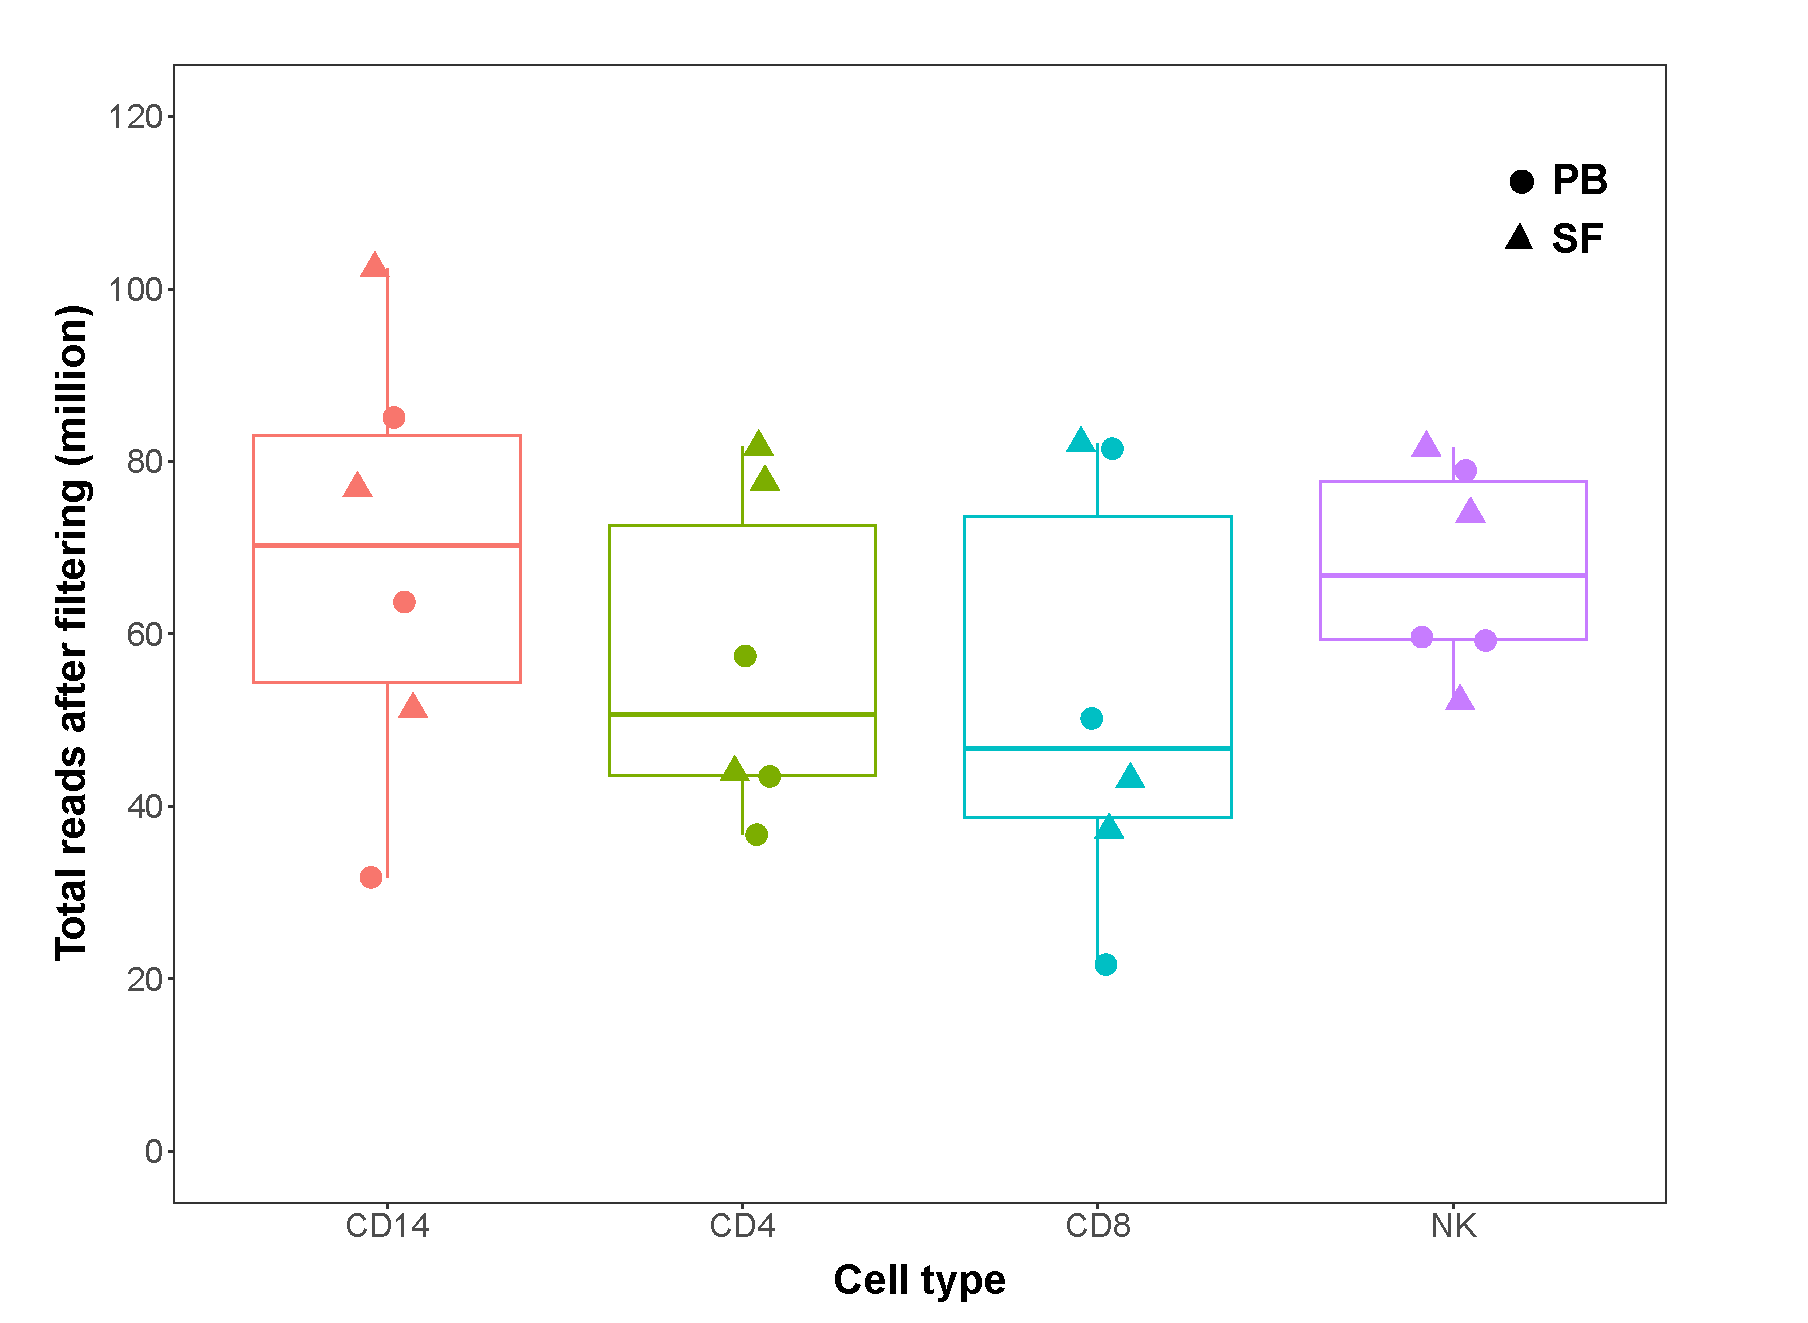
\includegraphics[width=\textwidth]{./Results3/pdfs/ATAC_PSA_total_filtered_reads_boxplot}
\caption{}
\end{subfigure}
~
\begin{subfigure}[b]{0.48\textwidth}
\centering 
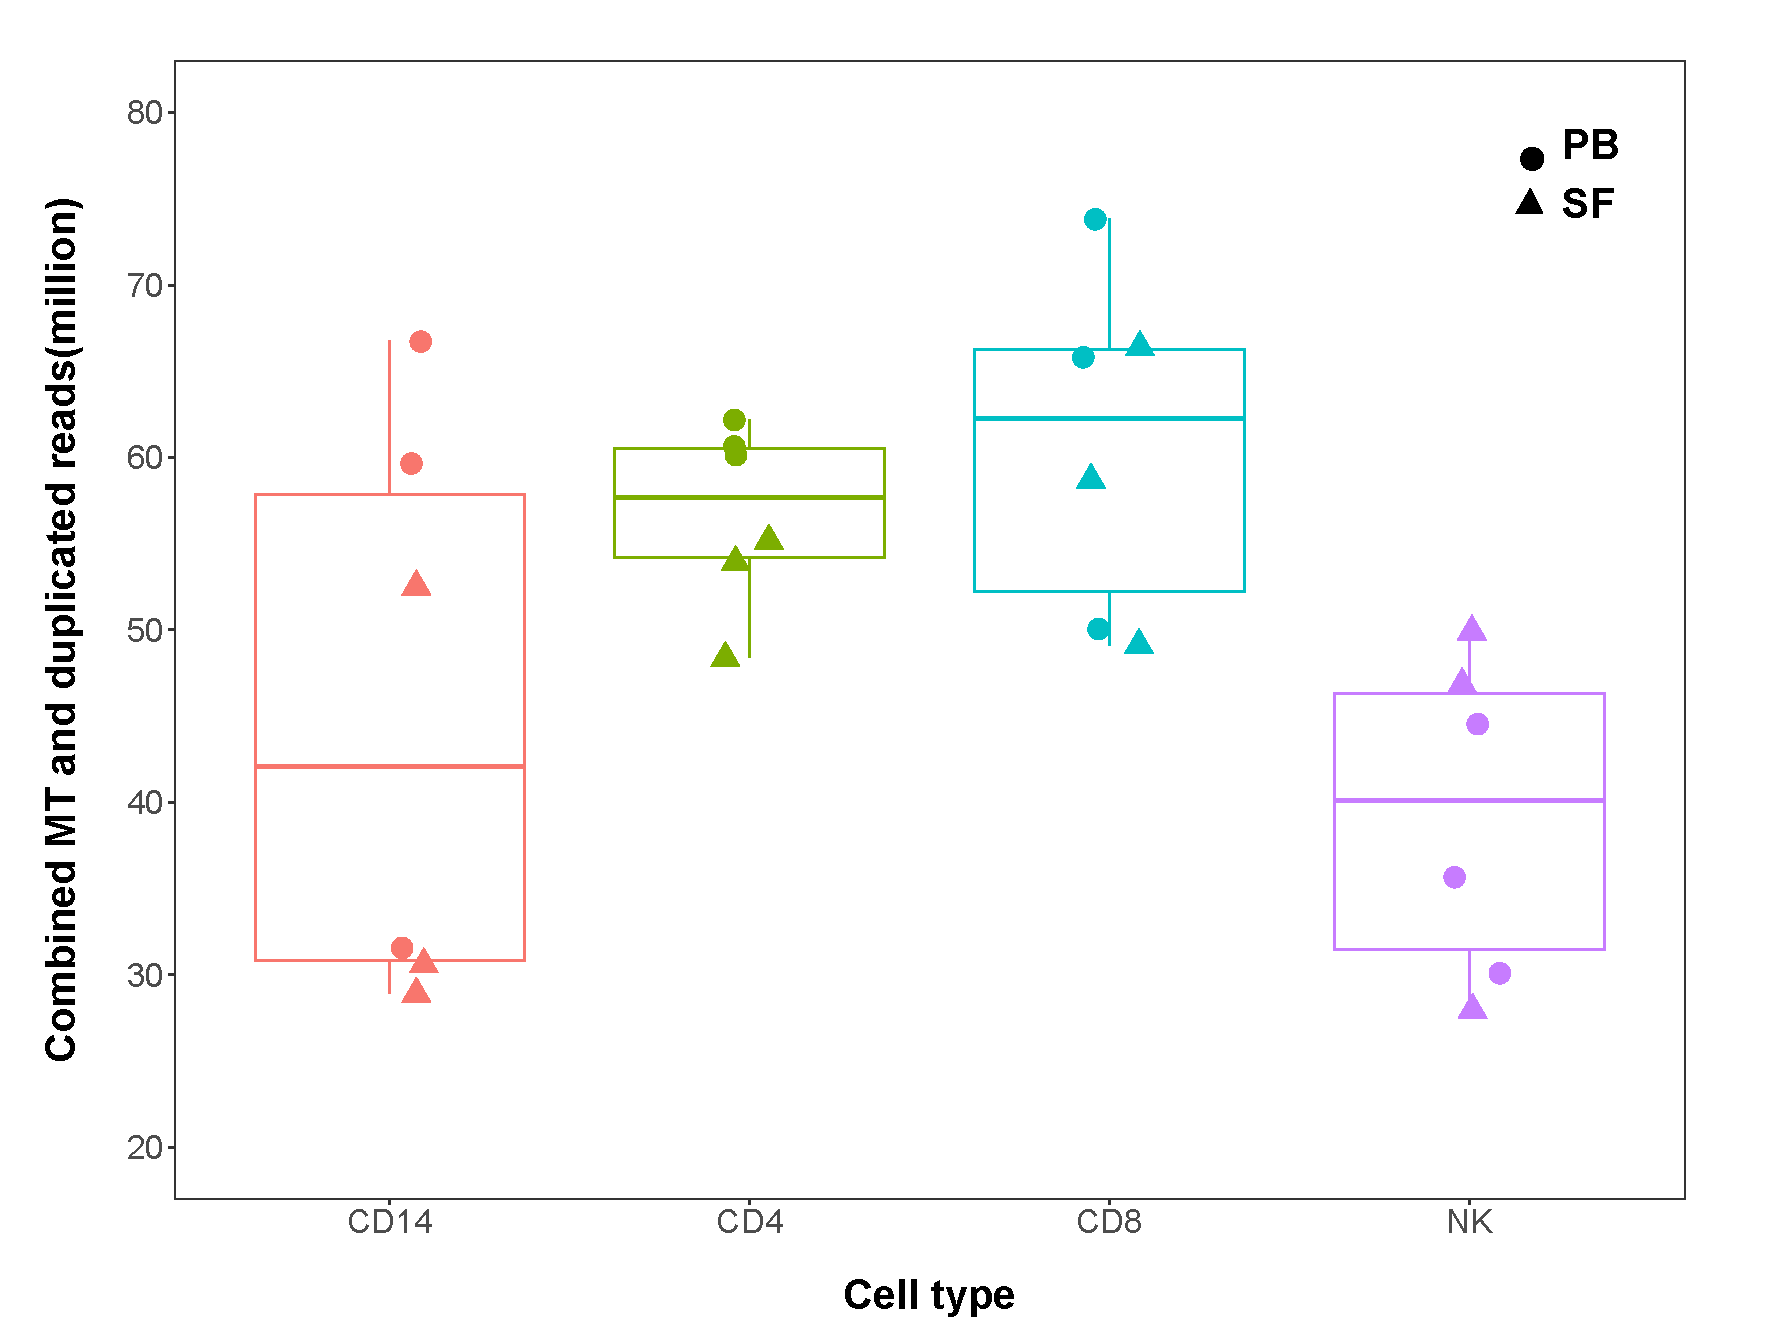
\includegraphics[width=\textwidth]{./Results3/pdfs/ATAC_PSA_pcnt_dups_and_MT_reads_boxplot}
\caption{}
\end{subfigure}
~
\begin{subfigure}[b]{0.48\textwidth} 
%the [b] prevents offset in subcaptions
\centering
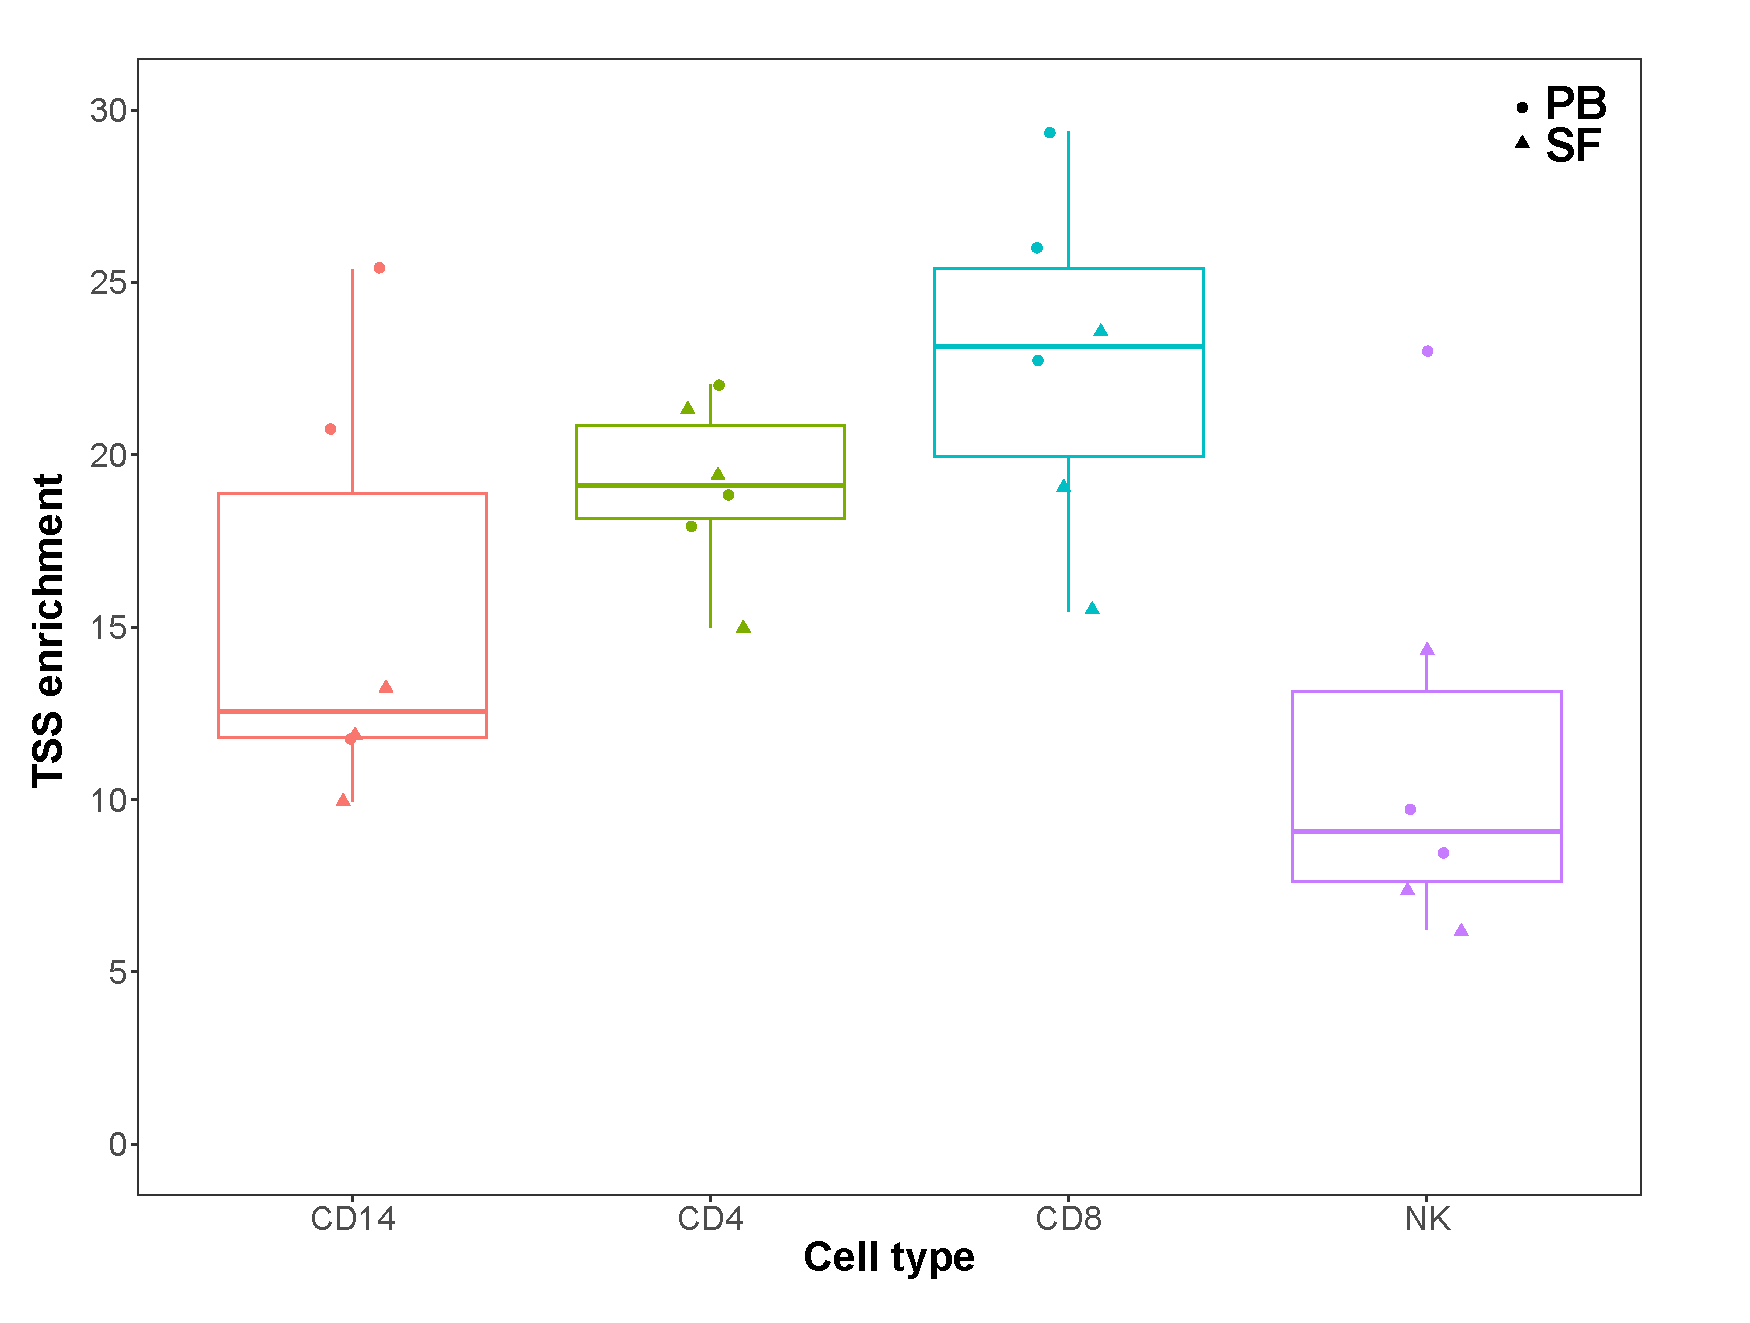
\includegraphics[width=\textwidth]{./Results3/pdfs/ATAC_PSA_all_TSS_max_per_cell_type}%
\caption{}
\end{subfigure}
\begin{subfigure}[b]{0.48\textwidth} 
%the [b] prevents offset in subcaptions
\centering
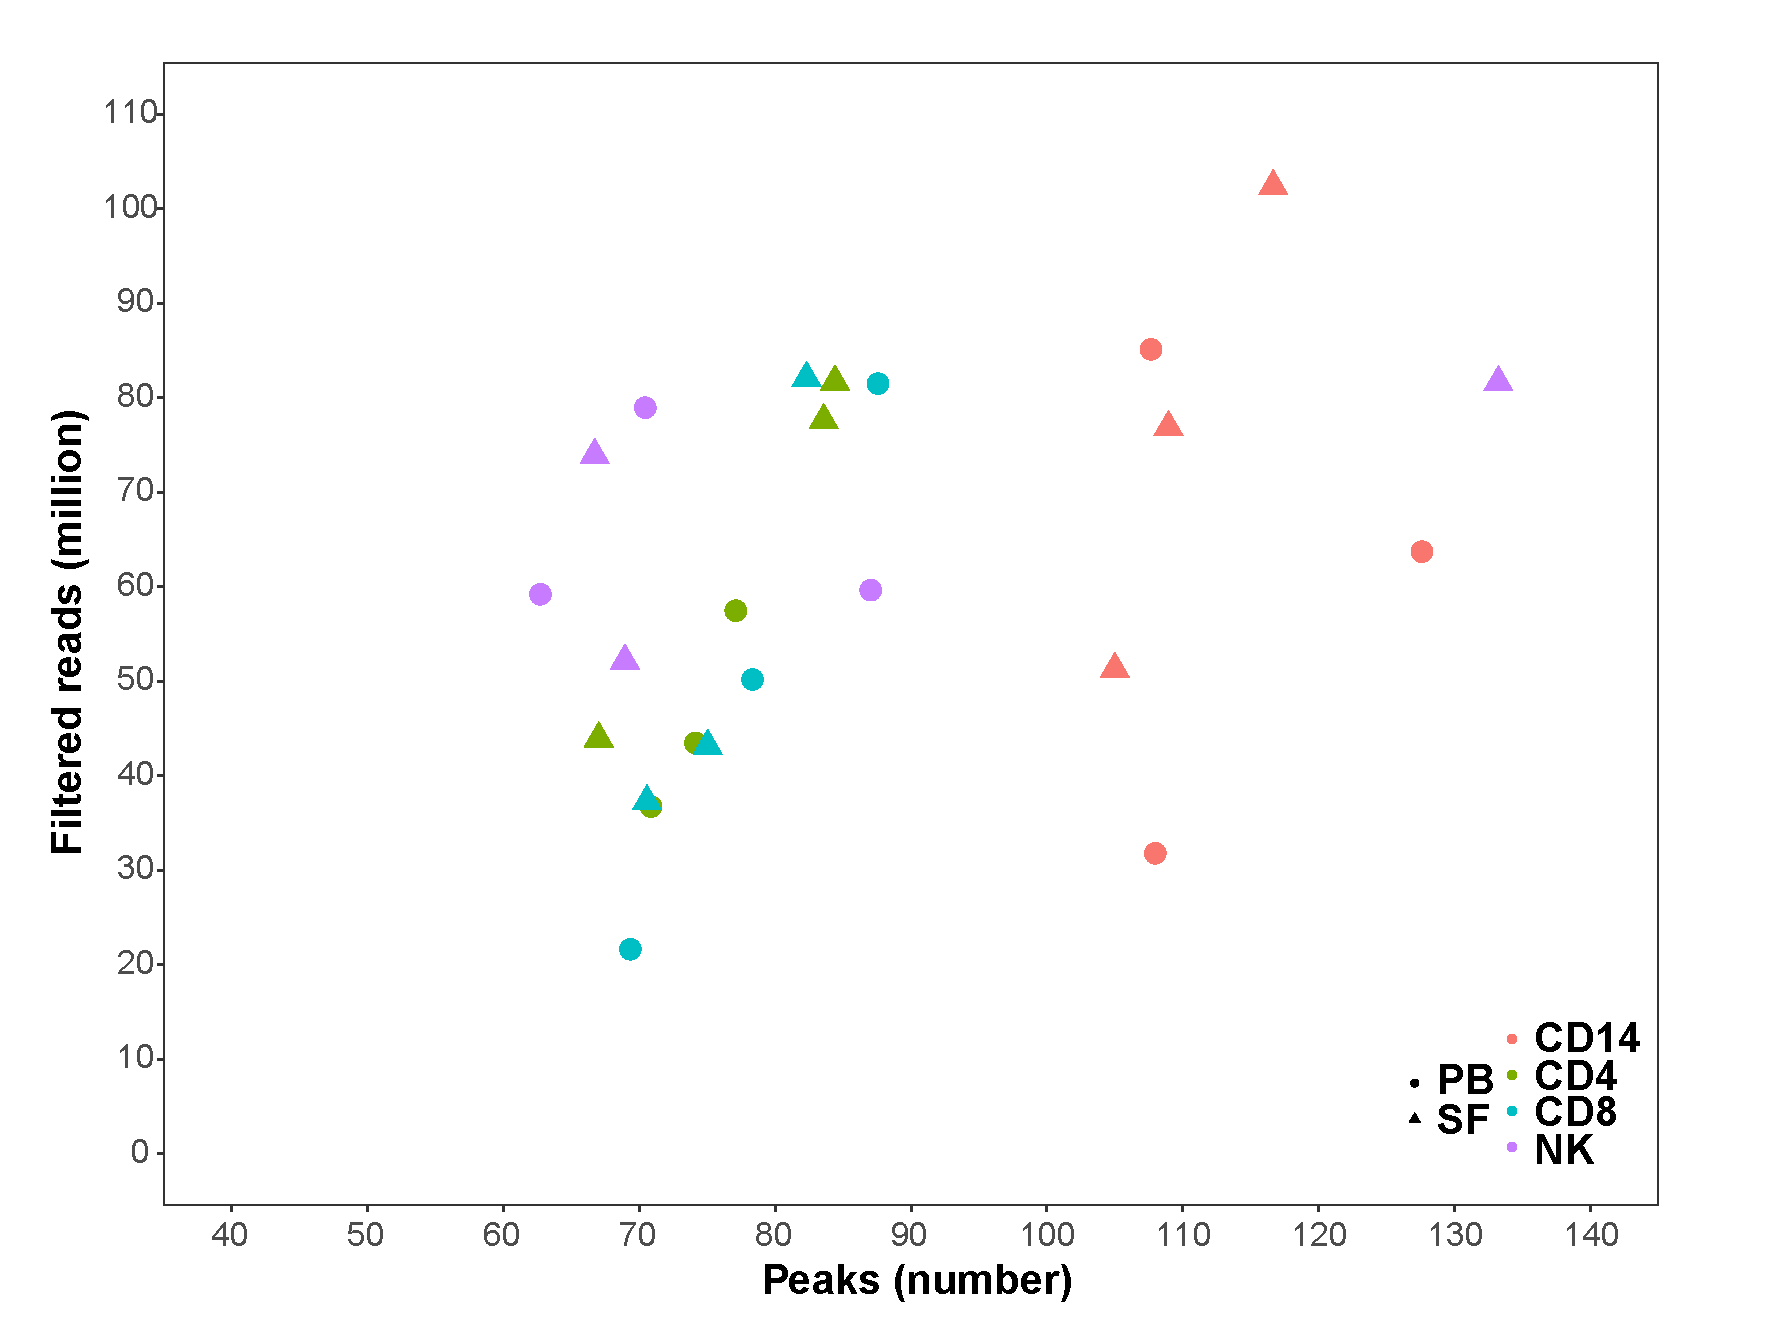
\includegraphics[width=\textwidth]{./Results3/pdfs/ATAC_PSA_all_peaks_vs_num_reads}%
\caption{}
\end{subfigure}
\caption[QC of FAST-ATAC PsA samples in four cell types]{\textbf{QC of FAST-ATAC PsA samples in four cell types}. }
\label{figure:PsA_FAST_ATAC_QC}
\end{figure}

When identifying open chromatin regions through peak calling and standard filtering for FDR$<$0.01 (not the IDR sample-specific filtering), the number of peaks ranged from $\sim$62$x10^3$ to $\sim$133$x10^3$ peaks per sample (Figure \ref{figure:PsA_FAST_ATAC_QC} d). A clear positive correlation between the number of called peaks and number of reads after filtering could be observed in the data. For example, CD14$^+$ was the cell type with greatest number of called peaks (108.4$x10^3$) as well as the greater median of reads remaining after filtering when compared to the other three cell types (Figure \ref{figure:PsA_FAST_ATAC_QC} a). For the NK, the two samples with the greatest TSS enrichment (PSA1718 SF and PB) showed greater number of called peaks when compared to the other NK samples with similar number of reads. This observation was consistent with the correlation between sample quality and the number of identified accessible chromatin regions previously demonstrated in Chapter \ref(ch:Results1).Overall, appropriate number of peaks were called in all the samples and no concerning outliers were identified.



\subsubsection{Open chromatin reflects cell type specificity and functional relevance }
In order to determine the ability of the open chromatin identified by the in house pipeline in the PsA sample cohort, a combined master list including all four cell types and the two tissues was built. Following Chapter \ref{ch:Mat} and Chapter \ref{ch:Results1}, the combined master list contained open chromatin regions identified in at least 30\% of the samples (in this case 7 samples) regardless cell type and tissue to avoid any bias.

\begin{figure}[H]
\centering
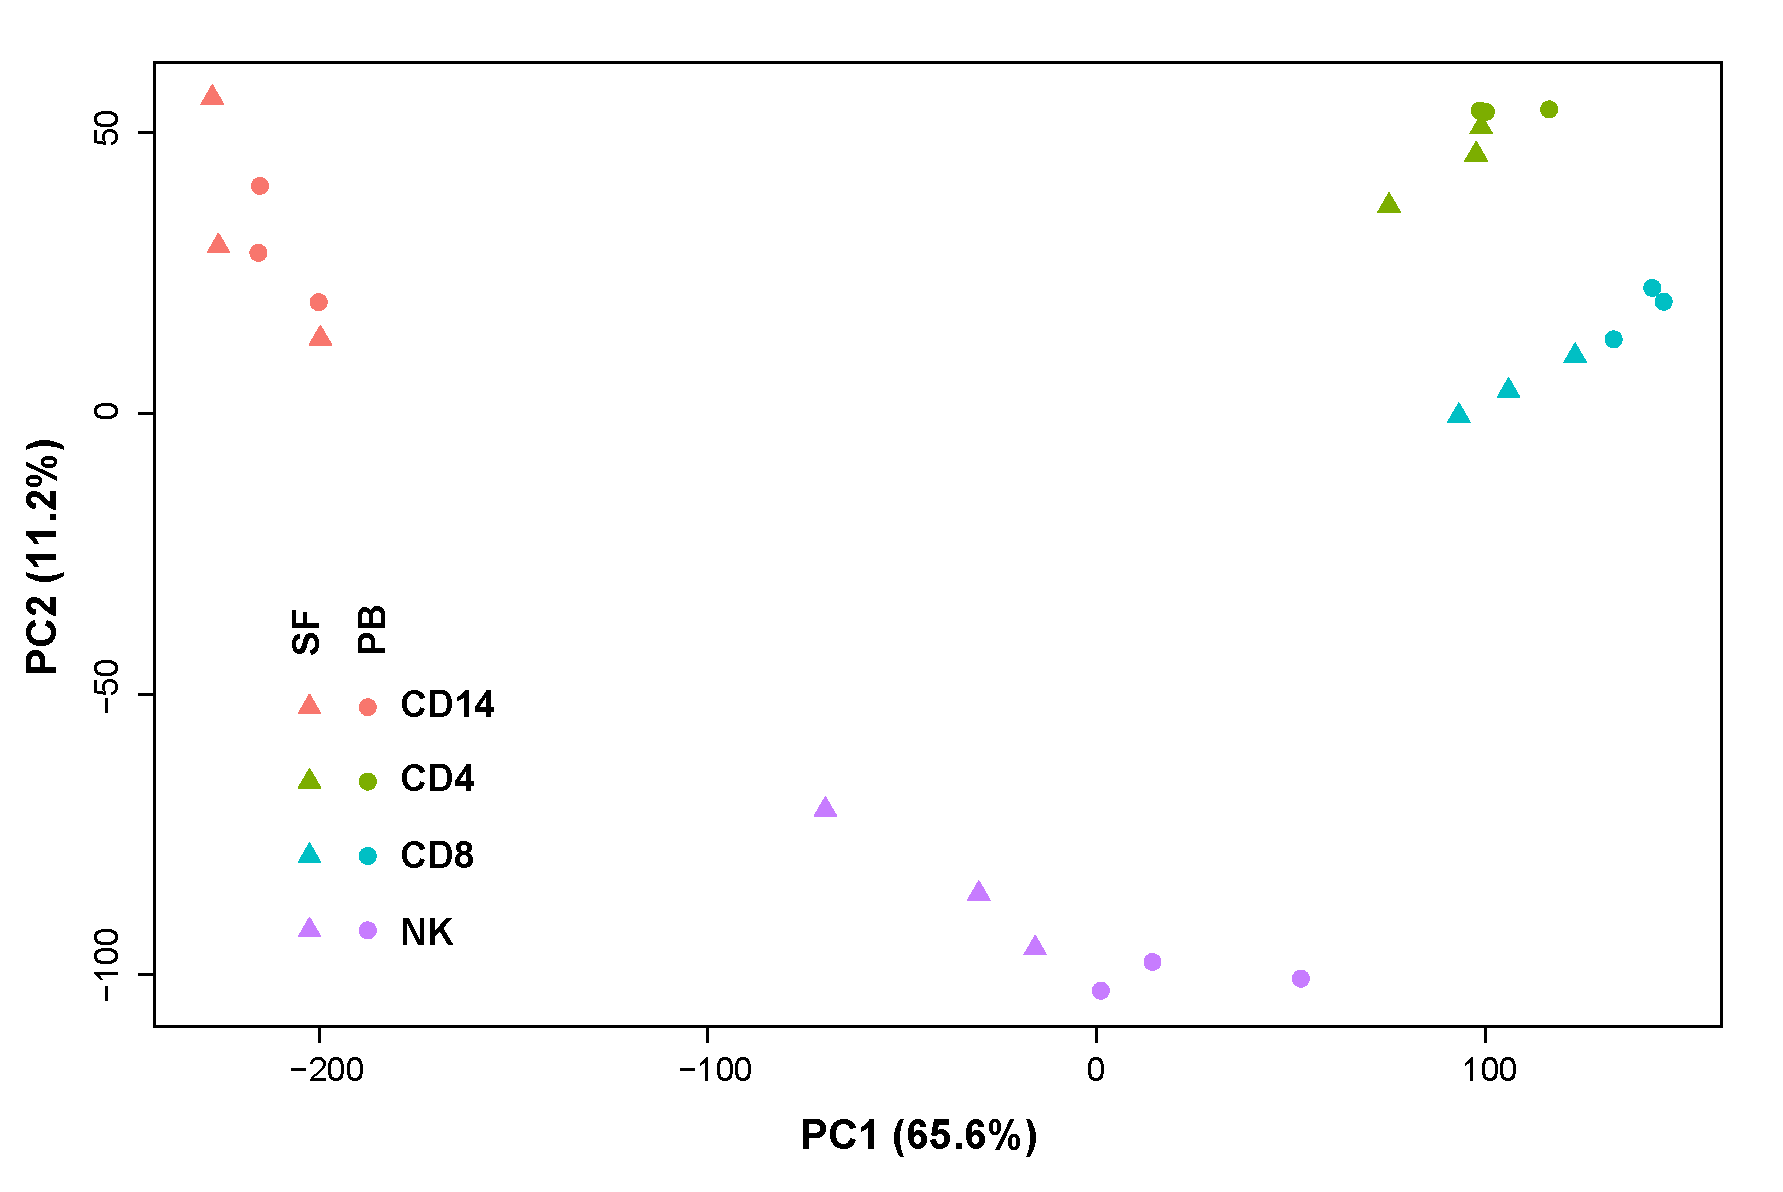
\includegraphics[width=0.7\textwidth]{./Results3/pdfs/ATAC_PSA_all_DESEq2_PCA}
\caption[Combined PCA analysis of all four cell types isolated from blood and SF.]{\textbf{Combined PCA analysis of all four cell types isolated from blood and SF.}}
\label{figure:PsA_FAST_ATAC_PCA}
\end{figure}



\bigskip
\begin{figure}[H]
\centering
\begin{subfigure}[b]{0.7\textwidth}
\centering 
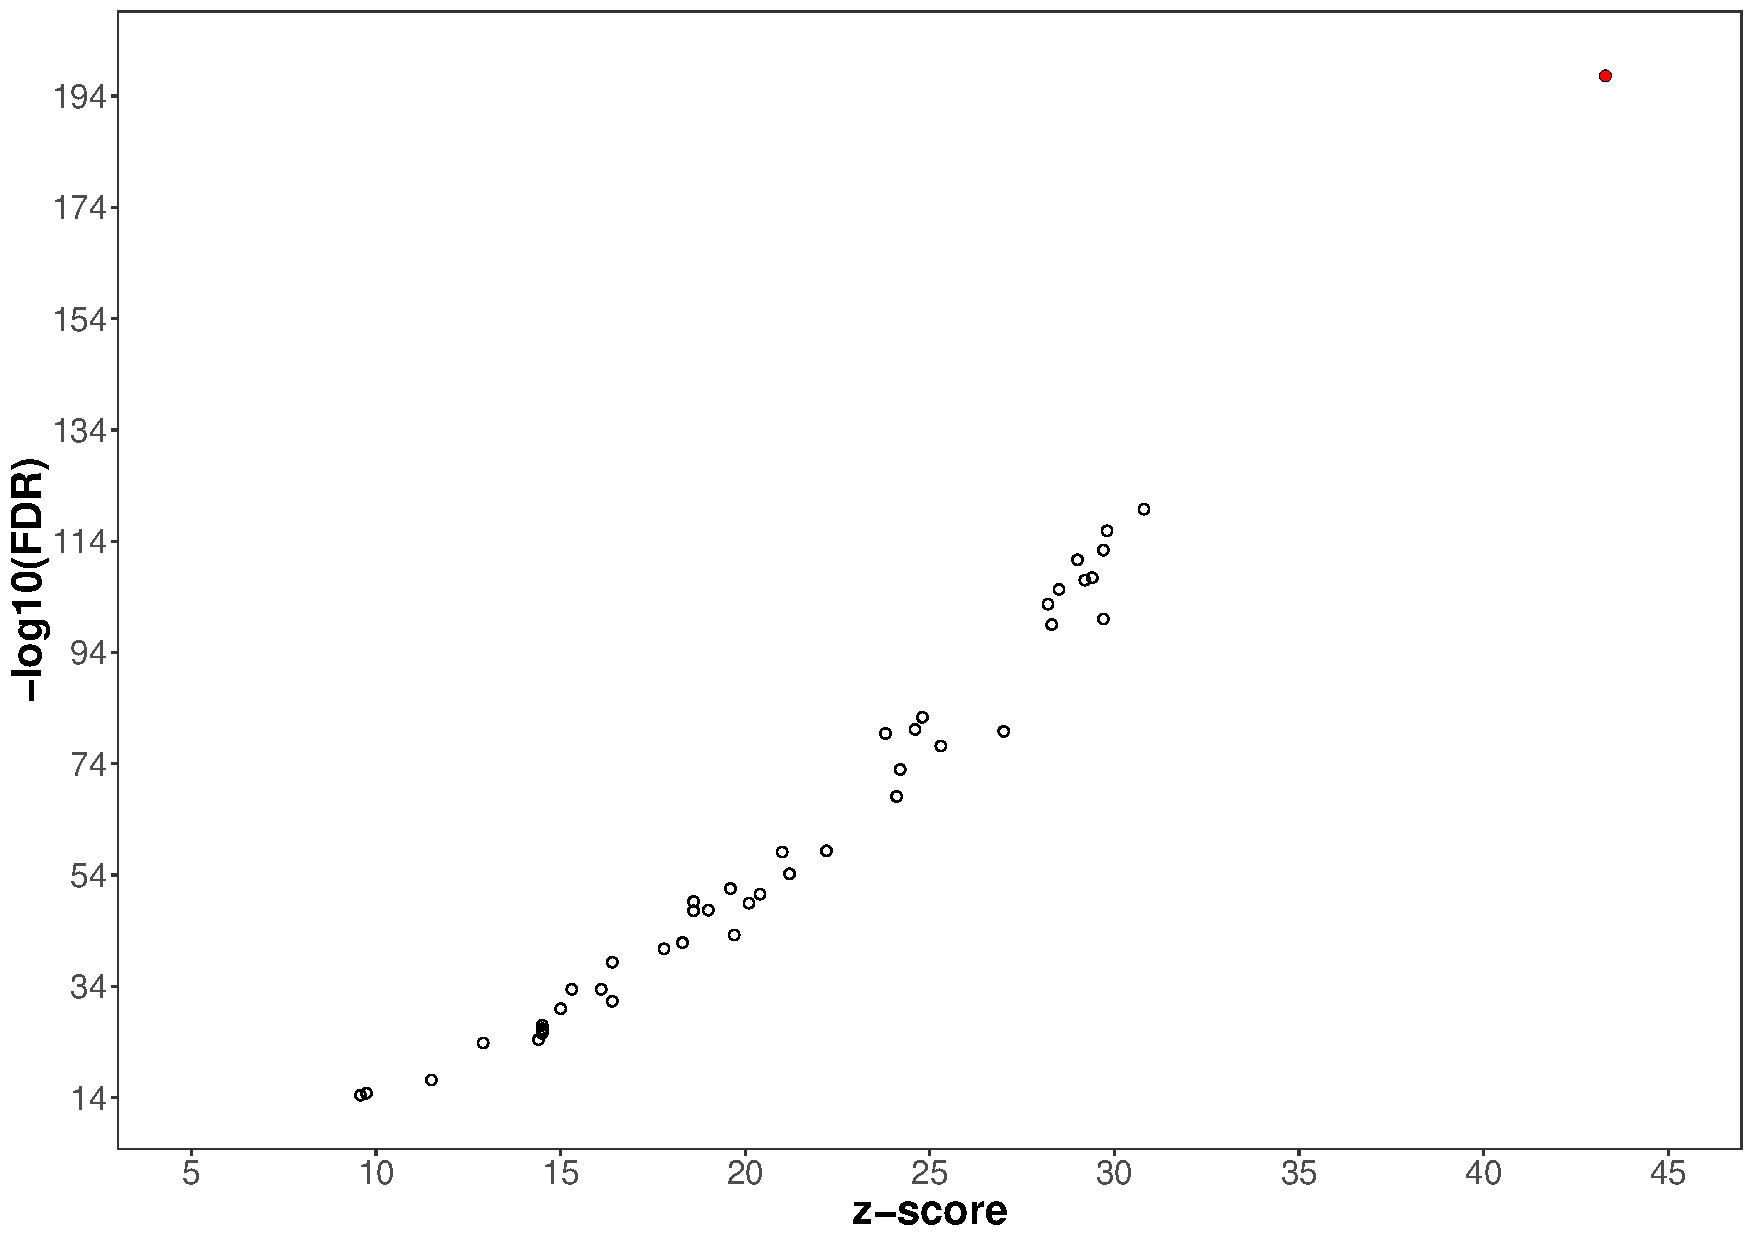
\includegraphics[width=\textwidth]{./Results3/pdfs/ATAC_PSA_all_GTeX_eQTL_enrichment_dotplot}
\caption{}
\end{subfigure}
~
\begin{subfigure}[b]{0.7\textwidth} 
%the [b] prevents offset in subcaptions
\centering
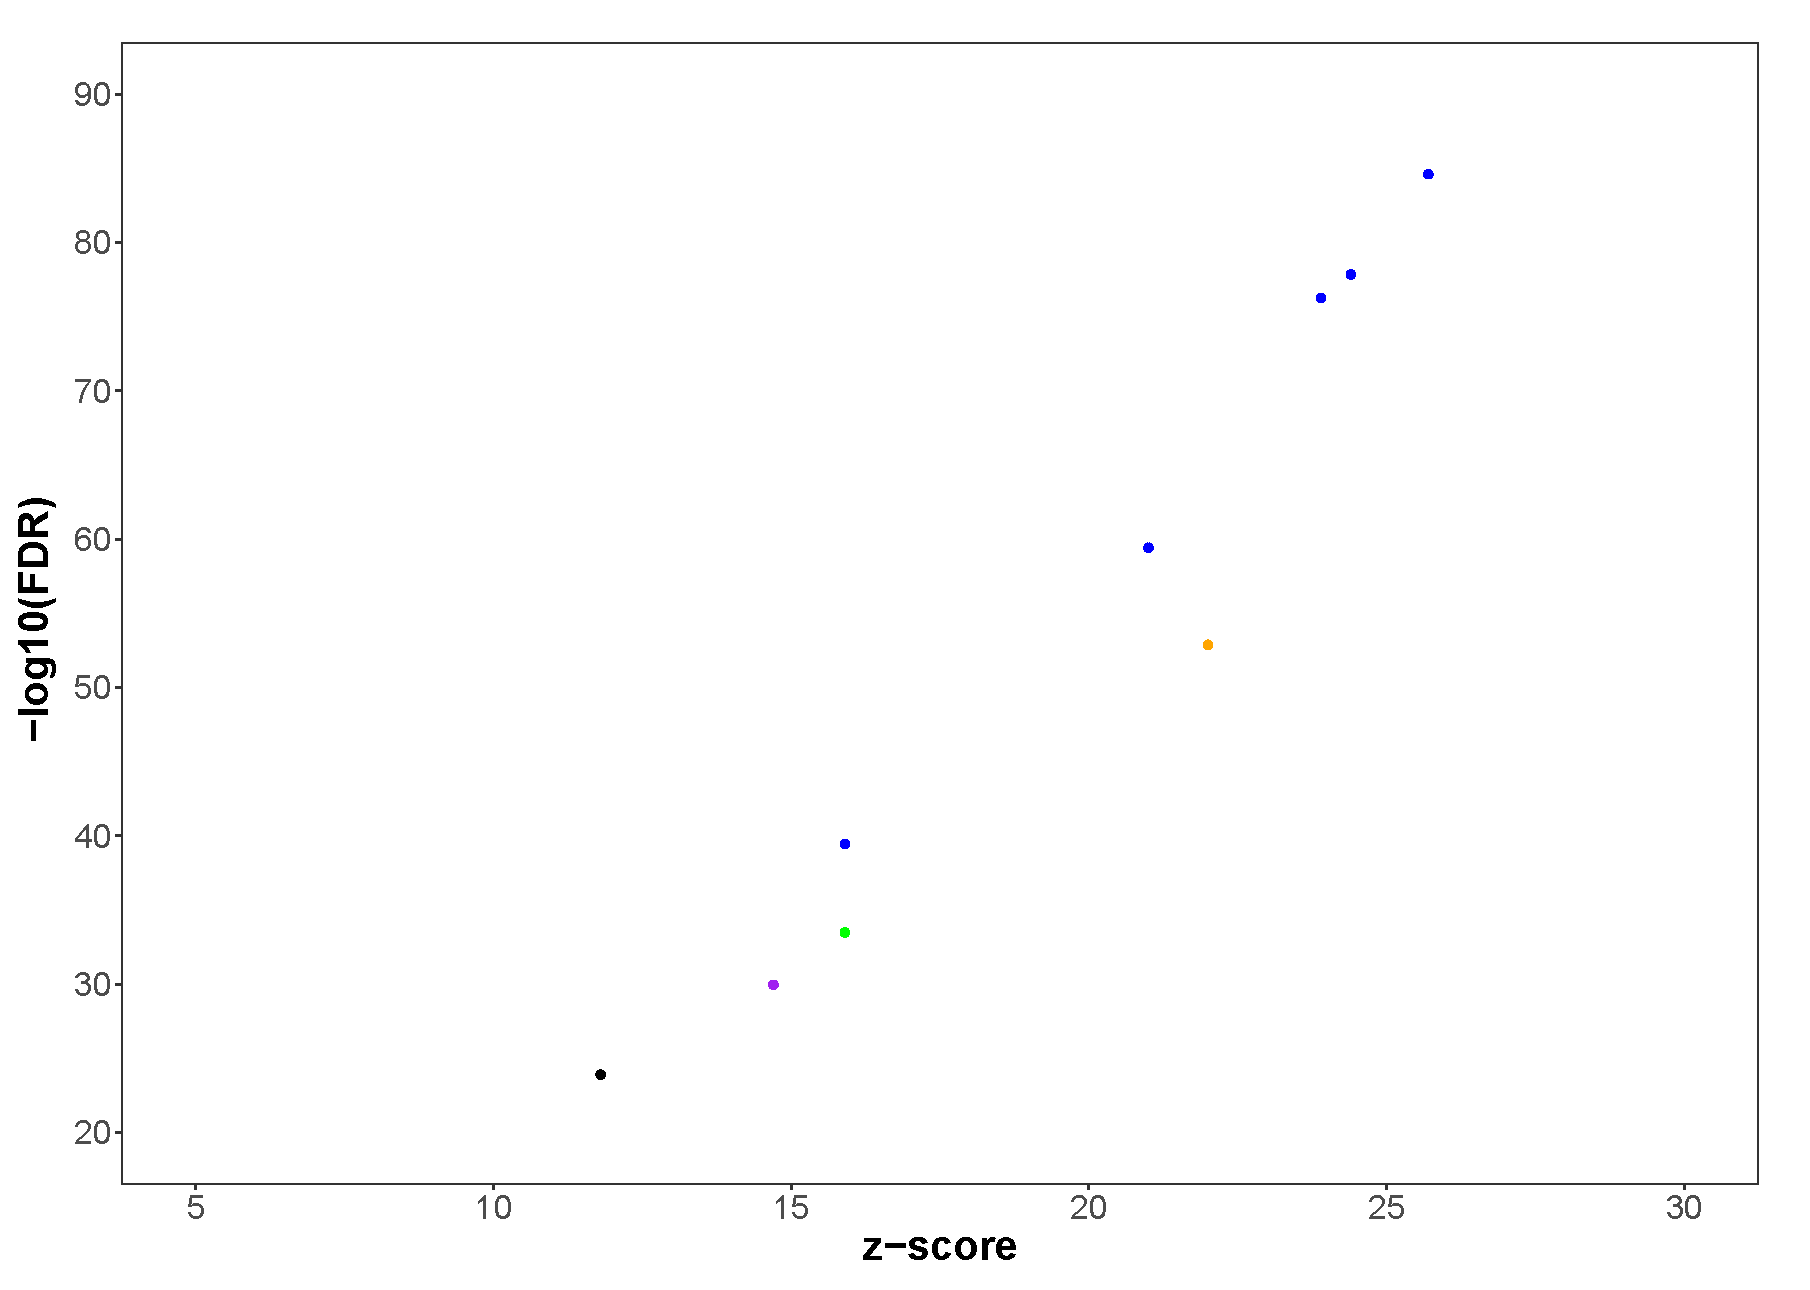
\includegraphics[width=\textwidth]{./Results3/pdfs/ATAC_PSA_all_Jknight_eQTL_enrichment_dotplot}
\caption{}
\end{subfigure}
\caption[Enrichment of eQTLs in the combined cell types PsA accessible chromatin master list.]{\textbf{Enrichment of eQTLs in the combined cell types PsA accessible chromatin master list} xxxx}
\label{figure:PsA_FAST_ATAC_eQTL_enrichment}
\end{figure}





\subsubsection{Differential open chromatin analysis between blood and SF}

Here I am planning an overview of the differential analysis including 
-total number of doc split between open in SF and open in PB,
-annotation according to chromatin accessibility in terms of all the hits
-mention how many of them are annotated in gene bodies and if more than one region within the same gene and choose an example of an interesting gene, include UCSC track showing the differences
-pathway enrichment analysis if possible per open chromatin in each cell type
-maybe include an A2 pathway which is different and unique between open in SF and PB in one cell type
-enrichment for TFBS and others, either global or per open in SF and PB,maybe combined plots for all cell types kind of fig6 of XGR paper


\begin{table}[htbp]
%\setlength{\tabcolsep}{20pt} only to stretch the columns if you want
%\renewcommand{\arraystretch}{1.5}
\centering
\begin{tabular}{@{} c c c c c}
\toprule
\textbf{Cell type} & \textbf{\% Total DOCs} &  \textbf{Proportion of DOCS (\%)} &\textbf{DOCs open in SF} & \textbf{DOCs open in PB} \\
\midrule
\midrule
CD14$^+$ & 5,285 & 23.3 & 3,779 & 1,506\\
CD4$^+$ & 1329 & 4.3 & 621 & 708\\
CD8$^+$ & 1570 & 4.5 &  & \\
NK      &  &  &  & \\
\bottomrule
\end{tabular}
\medskip %gap
\caption[Summary results of the chromatin accessibility analysis between SF and PB in PsA samples]{\textbf{xxxxxxxxx}}
\label{tab:PSA_DOCs_results}
\end{table}

\subsubsection{DOCs highlight relevant functional pathways in a cell type and tissue specific manner}


\subsection{Differential gene expression analysis in paired circulating and synovial immune cells}
Array data

%%%%%%%%%%%%%%%%%%%%%%%%%%%%%%%%%%%%%%%%%%%%%%%%%%
\section{Discussion}
%


fGWAS analysis as Matthias did would be of interest but needs appropriate GWAS data
I am going to try using XGR to do some of this 



